\documentclass[UTF8,12pt]{ctexart}
\usepackage[a4paper,margin=24mm]{geometry}
\usepackage{amsmath,amssymb,bm,graphicx,adjustbox}
\newcommand{\fitmath}[1]{\begin{adjustbox}{max width=\linewidth}$\displaystyle #1$\end{adjustbox}}
\setlength{\parindent}{0pt}
\setlength{\parskip}{.7em}
\sloppy
\allowdisplaybreaks
\begin{document}
\section*{2007 年考研数学三 · 真题}
\subsection*{2007年全国硕士研究生招生考试试题}

\subsection*{一、选择题（本题共10小题，每小题4分，满分40分）}

（1）当 \(\displaystyle x\to0^+\) 时，与 \(\displaystyle \sqrt x\) 等价的无穷小量是（　）。（A）\(\displaystyle 1-e^{\sqrt x}\)。（B）\(\displaystyle \ln(1+\sqrt x)\)。（C）\(\displaystyle \sqrt{1+\sqrt x}-1\)。（D）\(\displaystyle 1-\cos\sqrt x\)。


（2）设函数 \(\displaystyle f(x)\) 在 \(\displaystyle x=0\) 处连续，下列命题错误的是（　）。（A）若 \(\displaystyle \lim_{x\to0}\dfrac{\displaystyle f(x)}{\displaystyle x}\) 存在，则 \(\displaystyle f(0)=0\)。（B）若 \(\displaystyle \lim_{x\to0}\dfrac{\displaystyle f(x)+f(-x)}{\displaystyle x}\) 存在，则 \(\displaystyle f(0)=0\)。（C）若 \(\displaystyle \lim_{x\to0}\dfrac{\displaystyle f(x)}{\displaystyle x}\) 存在，则 \(\displaystyle f^{\prime}(0)\) 存在。（D）若 \(\displaystyle \lim_{x\to0}\dfrac{\displaystyle f(x)-f(-x)}{\displaystyle x}\) 存在，则 \(\displaystyle f^{\prime}(0)\) 存在。


（3）如图，连续函数 \(\displaystyle y=f(x)\) 在区间 \(\displaystyle [-3,\allowbreak -2]\)、\(\displaystyle [2,\allowbreak 3]\) 上的图形分别是直径为1的上、下半圆周，在区间 \(\displaystyle [-2,\allowbreak 0]\)、\(\displaystyle [0,\allowbreak 2]\) 上的图形分别是直径为2的下、上半圆周。设 \(\displaystyle F(x)=\displaystyle \int_0^xf(t)\,\mathrm dt\)，则下列结论正确的是（　）。


\begin{center}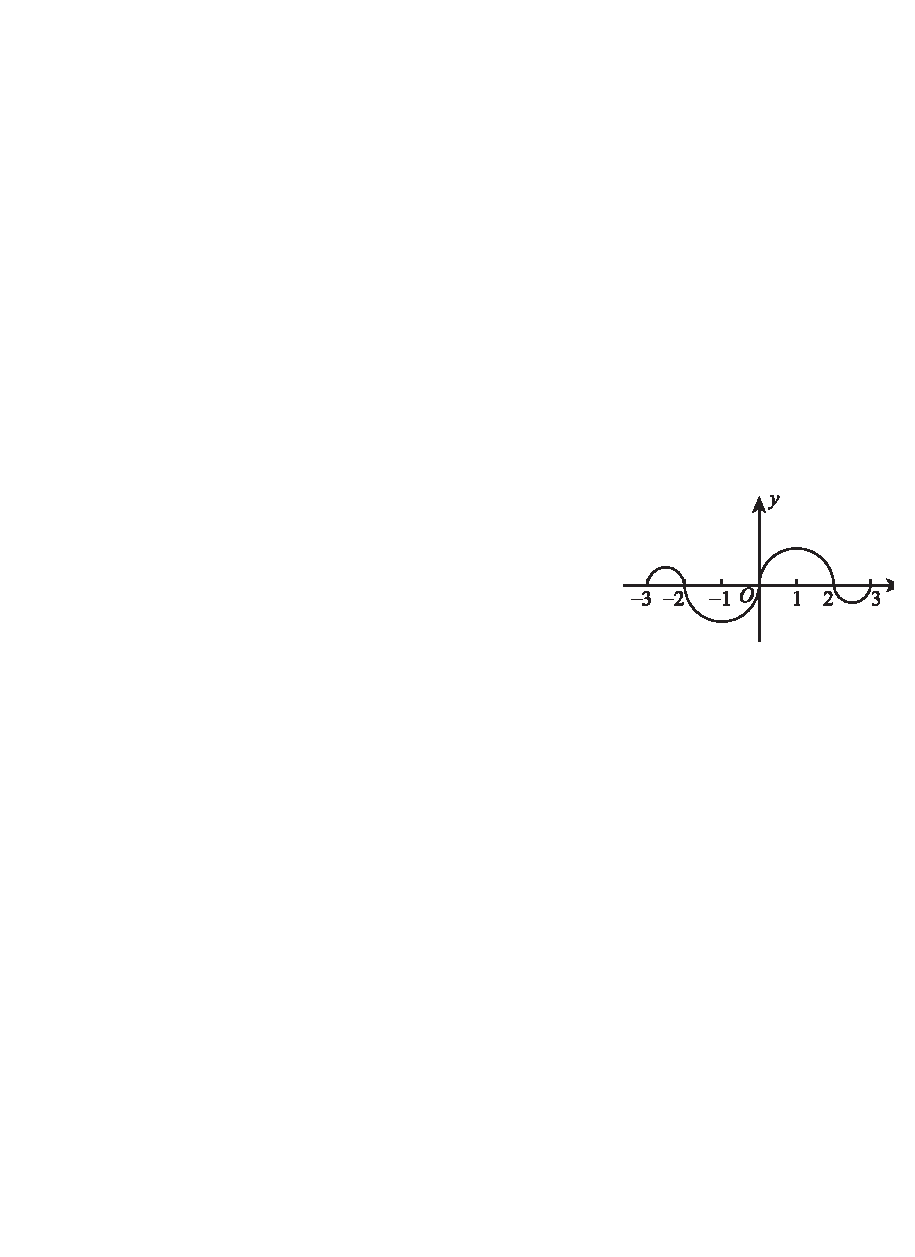
\includegraphics[width=.48\linewidth]{../assets/figures/page-110-05.pdf}\end{center}

（A）\(\displaystyle F(3)=-\dfrac{\displaystyle 3}{\displaystyle 4}F(-2)\)。（B）\(\displaystyle F(3)=\dfrac{\displaystyle 5}{\displaystyle 4}F(2)\)。（C）\(\displaystyle F(-3)=\dfrac{\displaystyle 3}{\displaystyle 4}F(2)\)。（D）\(\displaystyle F(-3)=-\dfrac{\displaystyle 5}{\displaystyle 4}F(-2)\)。


（4）设函数 \(\displaystyle f(x,\allowbreak y)\) 连续，则二次积分 \(\displaystyle \int_{\pi/2}^{\pi}\mathrm dx\displaystyle \int_{\sin x}^{1}f(x,\allowbreak y)\,\mathrm dy\) 等于（　）。（A）\(\displaystyle \int_0^1\mathrm dy\displaystyle \int_{\pi+\arcsin y}^{\pi}f(x,\allowbreak y)\,\mathrm dx\)。（B）\(\displaystyle \int_0^1\mathrm dy\displaystyle \int_{\pi-\arcsin y}^{\pi}f(x,\allowbreak y)\,\mathrm dx\)。（C）\(\displaystyle \int_0^1\mathrm dy\displaystyle \int_{\pi/2}^{\pi+\arcsin y}f(x,\allowbreak y)\,\mathrm dx\)。（D）\(\displaystyle \int_0^1\mathrm dy\displaystyle \int_{\pi/2}^{\pi-\arcsin y}f(x,\allowbreak y)\,\mathrm dx\)。


（5）设某商品的需求函数为 \(\displaystyle Q=160-2p\)，其中 \(\displaystyle Q,\allowbreak p\) 分别表示需求量和价格，如果该商品需求弹性的绝对值等于1，则商品的价格是（　）。（A）10。（B）20。（C）30。（D）40。


（6）曲线 \(\displaystyle y=\dfrac{\displaystyle 1}{\displaystyle x}+\ln(1+e^x)\) 渐近线的条数为（　）。（A）0。（B）1。（C）2。（D）3。


（7）设向量组 \(\displaystyle \alpha_1,\allowbreak \alpha_2,\allowbreak \alpha_3\) 线性无关，则下列向量组线性相关的是（　）。（A）\(\displaystyle \alpha_1-\alpha_2,\allowbreak \alpha_2-\alpha_3,\allowbreak \alpha_3-\alpha_1\)。（B）\(\displaystyle \alpha_1+\alpha_2,\allowbreak \alpha_2+\alpha_3,\allowbreak \alpha_3+\alpha_1\)。（C）\(\displaystyle \alpha_1-2\alpha_2,\allowbreak \alpha_2-2\alpha_3,\allowbreak \alpha_3-2\alpha_1\)。（D）\(\displaystyle \alpha_1+2\alpha_2,\allowbreak \alpha_2+2\alpha_3,\allowbreak \alpha_3+2\alpha_1\)。


（8）设矩阵 \(\displaystyle A=\begin{pmatrix}2&-1&-1\\-1&2&-1\\-1&-1&2\end{pmatrix}\)，\(\displaystyle B=\begin{pmatrix}1&0&0\\0&1&0\\0&0&0\end{pmatrix}\)，则 \(\displaystyle A\) 与 \(\displaystyle B\)（　）。（A）合同且相似。（B）合同，但不相似。（C）不合同，但相似。（D）既不合同，也不相似。


（9）某人向同一目标独立重复射击，每次射击命中目标的概率为 \(\displaystyle p\;(0<p<1)\)，则此人第4次射击恰好第2次命中目标的概率为（　）。（A）\(\displaystyle 3p(1-p)^2\)。（B）\(\displaystyle 6p(1-p)^2\)。（C）\(\displaystyle 3p^2(1-p)^2\)。（D）\(\displaystyle 6p^2(1-p)^2\)。


（10）设随机变量 \(\displaystyle (X,\allowbreak Y)\) 服从二维正态分布，且 \(\displaystyle X\) 与 \(\displaystyle Y\) 不相关，\(\displaystyle f_X(x),\allowbreak f_Y(y)\) 分别表示 \(\displaystyle X,\allowbreak Y\) 的概率密度，则在 \(\displaystyle Y=y\) 的条件下，\(\displaystyle X\) 的条件概率密度 \(\displaystyle f_{X\mid Y}(x\mid y)\) 为（　）。（A）\(\displaystyle f_X(x)\)。（B）\(\displaystyle f_Y(y)\)。（C）\(\displaystyle f_X(x)f_Y(y)\)。（D）\(\displaystyle \dfrac{\displaystyle f_X(x)}{\displaystyle f_Y(y)}\)。


\subsection*{二、填空题（本题共6小题，每小题4分，满分24分）}

（11）\(\displaystyle \lim_{x\to+\infty}\dfrac{\displaystyle x^3+x^2+1}{\displaystyle 2^x+x^3}(\sin x+\cos x)=\)\_\_\_\_\_\_。


（12）设函数 \(\displaystyle y=\dfrac{\displaystyle 1}{\displaystyle 2x+3}\)，则 \(\displaystyle y^{(n)}(0)=\)\_\_\_\_\_\_。


（13）设 \(\displaystyle f(u,\allowbreak v)\) 是二元可微函数，\(\displaystyle z=f(\dfrac{\displaystyle y}{\displaystyle x},\allowbreak \dfrac{\displaystyle x}{\displaystyle y})\)，则 \(\displaystyle x\dfrac{\displaystyle \partial z}{\displaystyle \partial x}-y\dfrac{\displaystyle \partial z}{\displaystyle \partial y}=\)\_\_\_\_\_\_。


（14）微分方程 \(\displaystyle \dfrac{\displaystyle \mathrm dy}{\displaystyle \mathrm dx}=\dfrac{\displaystyle y}{\displaystyle x}-\dfrac{\displaystyle 1}{\displaystyle 2}(\dfrac{\displaystyle y}{\displaystyle x})^3\) 满足 \(\displaystyle \left.y\right|_{x=1}=1\) 的特解为 \(\displaystyle y=\)\_\_\_\_\_\_。


（15）设矩阵 \(\displaystyle A=\begin{pmatrix}0&1&0&0\\0&0&1&0\\0&0&0&1\\0&0&0&0\end{pmatrix}\)，则 \(\displaystyle A^3\) 的秩为\_\_\_\_\_\_。


（16）在区间 \(\displaystyle (0,\allowbreak 1)\) 中随机地取两个数，则这两个数之差的绝对值小于 \(\displaystyle \dfrac{\displaystyle 1}{\displaystyle 2}\) 的概率为\_\_\_\_\_\_。


\subsection*{三、解答题（本题共8小题，满分86分。解答应写出文字说明、证明过程或演算步骤）}

（17）（本题满分10分）设函数 \(\displaystyle y=y(x)\) 由方程 \(\displaystyle y\ln y-x+y=0\) 确定，试判断曲线 \(\displaystyle y=y(x)\) 在点 \(\displaystyle (1,\allowbreak 1)\) 附近的凹凸性。


（18）（本题满分11分）设二元函数 \(\displaystyle f(x,\allowbreak y)=\begin{cases}x^2,\allowbreak &|x|+|y|\le1,\allowbreak \\\dfrac{\displaystyle 1}{\displaystyle \sqrt{x^2+y^2}},\allowbreak &1<|x|+|y|\le2,\allowbreak \end{cases}\) 计算二重积分 \(\displaystyle \iint_Df(x,\allowbreak y)\,\mathrm d\sigma\)，其中 \(\displaystyle D=\{(x,\allowbreak y)\mid |x|+|y|\le2\}\)。


（19）（本题满分10分）设函数 \(\displaystyle f(x),\allowbreak g(x)\) 在 \(\displaystyle [a,\allowbreak b]\) 上连续，在 \(\displaystyle (a,\allowbreak b)\) 内二阶可导且存在相等的最大值，又 \(\displaystyle f(a)=g(a)\)，\(\displaystyle f(b)=g(b)\)。证明：（I）存在 \(\displaystyle \eta\in(a,\allowbreak b)\)，使得 \(\displaystyle f(\eta)=g(\eta)\)；（II）存在 \(\displaystyle \xi\in(a,\allowbreak b)\)，使得 \(\displaystyle f^{\prime\prime}(\xi)=g^{\prime\prime}(\xi)\)。


（20）（本题满分11分）将函数 \(\displaystyle f(x)=\dfrac{\displaystyle 1}{\displaystyle x^2-3x-4}\) 展开成 \(\displaystyle x-1\) 的幂级数，并指出其收敛区间。


（21）（本题满分11分）设线性方程组\textcircled{1} \(\displaystyle \begin{cases}x_1+x_2+x_3=0,\allowbreak \\x_1+2x_2+ax_3=0,\allowbreak \\x_1+4x_2+a^2x_3=0,\allowbreak \end{cases}\) 与方程组\textcircled{2} \(\displaystyle x_1+2x_2+x_3=a-1\) 有公共解，求 \(\displaystyle a\) 的值及所有公共解。


（22）（本题满分11分）设3阶实对称矩阵 \(\displaystyle A\) 的特征值 \(\displaystyle \lambda_1=1,\allowbreak \lambda_2=2,\allowbreak \lambda_3=-2\)，且 \(\displaystyle \alpha_1=(1,\allowbreak -1,\allowbreak 1)^{\mathrm T}\) 是 \(\displaystyle A\) 的属于 \(\displaystyle \lambda_1\) 的一个特征向量。记 \(\displaystyle B=A^5-4A^3+E\)，其中 \(\displaystyle E\) 为3阶单位矩阵。（I）验证 \(\displaystyle \alpha_1\) 是矩阵 \(\displaystyle B\) 的特征向量，并求 \(\displaystyle B\) 的全部特征值与特征向量；（II）求矩阵 \(\displaystyle B\)。


（23）（本题满分11分）设二维随机变量 \(\displaystyle (X,\allowbreak Y)\) 的概率密度为 \(\displaystyle f(x,\allowbreak y)=\begin{cases}2-x-y,\allowbreak &0<x<1,\allowbreak \ 0<y<1,\allowbreak \\0,\allowbreak &\text{其他}.\end{cases}\)（I）求 \(\displaystyle P\{X>2Y\}\)；（II）求 \(\displaystyle Z=X+Y\) 的概率密度 \(\displaystyle f_Z(z)\)。


（24）（本题满分11分）设总体 \(\displaystyle X\) 的概率密度为 \(\displaystyle f(x;\theta)=\begin{cases}\dfrac{\displaystyle 1}{\displaystyle 2\theta},\allowbreak &0<x<\theta,\allowbreak \\\dfrac{\displaystyle 1}{\displaystyle 2(1-\theta)},\allowbreak &\theta\le x<1,\allowbreak \\0,\allowbreak &\text{其他},\allowbreak \end{cases}\) 其中参数 \(\displaystyle \theta\;(0<\theta<1)\) 未知，\(\displaystyle X_1,\allowbreak X_2,\allowbreak \ldots,\allowbreak X_n\) 是来自总体 \(\displaystyle X\) 的简单随机样本，\(\displaystyle \bar X\) 是样本均值。（I）求参数 \(\displaystyle \theta\) 的矩估计量 \(\displaystyle \hat\theta\)；（II）（超纲题）判断 \(\displaystyle 4\bar X^2\) 是否为 \(\displaystyle \theta^2\) 的无偏估计量，并说明理由。（无偏估计为超纲概念，可改为“验证是否有 \(\displaystyle E(4\bar X^2)=\theta^2\)”）

\end{document}
